\section{Convex Functions}
\subsection{Solved exercises}
\subsubsection{CO: 3.2}
\textbf{Some level sets of a function $f$ are shown below. The curve labeled 1 shows $\{x | f(x) = 1\}$}, etc.
\begin{figure}[H]
    \centering
    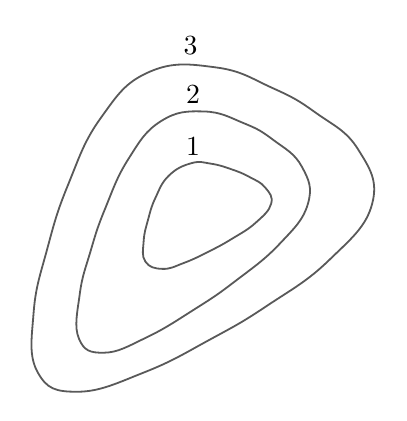
\begin{tikzpicture}[x=1.05cm,y=1.05cm]
        \tikzset{level curve/.style={draw=black!65, line width=0.65pt}}

        % On the right, successive level curves become farther apart.  Thus
% equal increases in the level value occur over increasing distances.
\draw[level curve]
    plot[smooth cycle, tension=0.75] coordinates {
        (2.047,0.000) (1.526,-0.682) (0.774,-1.235)
        (0.090,-1.640) (-0.699,-2.035) (-1.515,-2.274)
        (-1.998,-2.040) (-2.048,-1.318) (-1.882,-0.542)
        (-1.630,0.232) (-1.235,1.038) (-0.650,1.594)
        (0.156,1.649) (0.836,1.402) (1.361,1.103)
        (1.877,0.657)
    };

\draw[level curve]
    plot[smooth cycle, tension=0.75] coordinates {
        (1.270,0.000) (0.926,-0.487) (0.378,-0.946)
        (-0.112,-1.283) (-0.684,-1.618) (-1.197,-1.802)
        (-1.500,-1.631) (-1.490,-1.094) (-1.361,-0.580)
        (-1.186,-0.067) (-0.901,0.542) (-0.507,0.999)
        (0.010,1.116) (0.494,0.974) (0.852,0.771)
        (1.196,0.449)
    };

\draw[level curve]
    plot[smooth cycle, tension=0.75] coordinates {
        (0.825,0.000) (0.639,-0.229) (0.358,-0.420)
        (0.073,-0.577) (-0.230,-0.716) (-0.489,-0.788)
        (-0.696,-0.700) (-0.717,-0.453) (-0.664,-0.194)
        (-0.575,0.070) (-0.412,0.340) (-0.141,0.490)
        (0.099,0.484) (0.344,0.417) (0.562,0.324)
        (0.754,0.195)
    };


        \node at (-0.12,0.69) {$1$};
        \node at (-0.12,1.32) {$2$};
        \node at (-0.15,1.91) {$3$};
    \end{tikzpicture}
    \caption{The first family of level curves in Exercise 3.2.}
    \label{fig:exercise-3-2-level-sets-a}
\end{figure}

\input{figures/exercise-3-2-level-sets-b.tex}

For the first family of curves seen in Figure \ref{fig:exercise-3-2-level-sets-a}, we can first conclude that they are certainly not concave or quasiconcave since the superlevel sets are not convex.
The sublevel sets are however convex so we can claim quasiconvexity. 
Recall the restriction of a convex function to any line through it's domain must also be convex, therefore to check convexity of $f$ we probe it's behavior along lines in the domain.
As is shown in Figure \ref{fig:exercise-3-2-level-sets-a-solution}, it is easy to identify directions in which the slope tapers off,
i.e. directions in which the graph lies above the chord between some points on the line. 
Therefore we can label any function with the level curves as shown in Figure \ref{fig:exercise-3-2-level-sets-a} as quasiconvex, but not convex, quasiconcave or concave.

Now for Figure \ref{fig:exercise-3-2-level-sets-b} we see that the superlevel sets are convex and the sublevel sets are not, so here it is the other way around.
Performing the same kind of analysis along lines in the domain, one draws the conclusion that this function is not only quasiconcave but actually concave as well.
So functions with the level curves shown in Figure \ref{fig:exercise-3-2-level-sets-b} are convcave and quasiconcave but neither convex nor quasiconvex. 

\medskip

\begin{figure}[H]
    \centering
    \begin{tikzpicture}[>=Latex]
        \tikzset{
            level curve/.style={draw=black!45, line width=0.55pt},
            concave slice/.style={draw=red!70!black, line width=0.9pt}
        }

        % The level curves and the concave-looking ray in x-space.
        \begin{scope}[x=0.92cm,y=0.92cm]
            % On the right, successive level curves become farther apart.  Thus
% equal increases in the level value occur over increasing distances.
\draw[level curve]
    plot[smooth cycle, tension=0.75] coordinates {
        (2.047,0.000) (1.526,-0.682) (0.774,-1.235)
        (0.090,-1.640) (-0.699,-2.035) (-1.515,-2.274)
        (-1.998,-2.040) (-2.048,-1.318) (-1.882,-0.542)
        (-1.630,0.232) (-1.235,1.038) (-0.650,1.594)
        (0.156,1.649) (0.836,1.402) (1.361,1.103)
        (1.877,0.657)
    };

\draw[level curve]
    plot[smooth cycle, tension=0.75] coordinates {
        (1.270,0.000) (0.926,-0.487) (0.378,-0.946)
        (-0.112,-1.283) (-0.684,-1.618) (-1.197,-1.802)
        (-1.500,-1.631) (-1.490,-1.094) (-1.361,-0.580)
        (-1.186,-0.067) (-0.901,0.542) (-0.507,0.999)
        (0.010,1.116) (0.494,0.974) (0.852,0.771)
        (1.196,0.449)
    };

\draw[level curve]
    plot[smooth cycle, tension=0.75] coordinates {
        (0.825,0.000) (0.639,-0.229) (0.358,-0.420)
        (0.073,-0.577) (-0.230,-0.716) (-0.489,-0.788)
        (-0.696,-0.700) (-0.717,-0.453) (-0.664,-0.194)
        (-0.575,0.070) (-0.412,0.340) (-0.141,0.490)
        (0.099,0.484) (0.344,0.417) (0.562,0.324)
        (0.754,0.195)
    };


            \draw[concave slice,->]
                (0.35,0) -- (2.38,0)
                node[right,black] {$\ell_{\mathrm{conc}}$};
            \foreach \x/\lev in {
                0.825/1,
                1.270/2,
                2.047/3
            } {
                \fill[red!70!black] (\x,0) circle (1.55pt)
                    node[below,black,font=\scriptsize] {$\lev$};
            }
        \end{scope}

        % Linear interpolation of the samples along the ray.
        \begin{scope}[xshift=5.0cm,yshift=-1.55cm,x=2.4cm,y=0.72cm]
            \draw[->] (-0.08,0.70) -- (1.42,0.70)
                node[below] {$s$};
            \draw[->] (-0.08,0.70) -- (-0.08,3.38)
                node[left] {$f$};
            \foreach \y in {1,2,3} {
                \draw (-0.10,\y) -- (-0.06,\y);
                \node[anchor=east,font=\scriptsize] at (-0.12,\y) {$\y$};
            }
            \draw[black!20,densely dotted] (0,0.70) -- (0,1);
            \draw[black!20,densely dotted] (0.445,0.70) -- (0.445,2);
            \draw[black!20,densely dotted] (1.222,0.70) -- (1.222,3);
            \draw[concave slice] (0,1) -- (0.445,2) -- (1.222,3);
            \foreach \x/\y in {0/1,0.445/2,1.222/3} {
                \fill[red!70!black] (\x,\y) circle (1.55pt);
            }
            \node[font=\scriptsize] at (0.67,3.52)
                {decreasing secant slopes};
        \end{scope}
    \end{tikzpicture}
    \caption{Linear interpolation of the sampled values along
        $\ell_{\mathrm{conc}}$.  Its decreasing secant slopes rule out
        convexity.}
    \label{fig:exercise-3-2-level-sets-a-solution}
\end{figure}

